\documentclass[12pt]{article}
\usepackage{color}
\usepackage{cite}
\usepackage{geometry}                % See geometry.pdf to learn the layout options. There are lots.
%\usepackage{pdflscape}        %single page landscape
                                %mode \begin{landscape} \end{landscape}
\geometry{letterpaper}                   % ... or a4paper or a5paper or ... 
%\usepackage[parfill]{parskip}    % Activate to begin paragraphs with an empty line rather than an indent
\usepackage{graphicx}
\usepackage{amssymb}
\usepackage{Sweave}
\newcommand{\etal}{\textit{et al.}}
\usepackage{hyperref}  %\hyperref[label_name]{''link text''}
                       %\hyperlink{label}{anchor caption}
                       %\hypertarget{label}{link caption}
\linespread{1.5}

\title{Dissertation Committee Meeting Spring 2012}
\author{M.K. Lau}
%\date{}                                           % Activate to display a given date or no date

\begin{document}
\maketitle

\thispagestyle{empty}

\setcounter{tocdepth}{3}  %%activate to number sections
\tableofcontents

\section{Meeting Outline (Max 2hrs)}
\begin{itemize}
\item Overview of dissertation goal 
\item Requirements
\item Projects 
\item Time-line 
\item Discussion
\end{itemize}

\section{Dissertation Goal}
Interactions among species contribute to both ecological and
evolutionary dynamics in ecosystems. Community genetics, which seeks
to identify the community-wide influence of genetic variation, has
primarily focused on the effects of focal species, typically
foundation species (i.e. dominant and keystone species). This
dissertation will aim to expand this scope to a larger number of
species in the community primarily through the integration of network
theory and community genetics.

\section{Requirements}

\subsection{Forms/Paperwork}

\begin{itemize}
\item \textbf{May 2012} Assessment, prospectus review and course plan approval
  \subitem Bio form 5 - PhD Program Form
  \subitem Bio form 10 - Progress/Funding Assessment
  \subitem Bio form 13 - Teaching requirement documentation
  \subitem Bio form 14 - Scientific paper presentation documentation
%\item \textbf{Oct 2012} Grant and written exam approval
\item \textbf{October 2012} Prospectus defense and oral exam
  \subitem Bio form 7 - Written exam results
  \subitem Bio form 10 - Progress/Funding Assessment
  \subitem Bio form 8 - Oral exam results REPORT
  \subitem Bio form 8.11a - Oral exam assessment/questionnaire
  \subitem Bio form 9 - Prospectus approval form
  \subitem Bio form 11 - Oral exam results
  \subitem Bio form 10 - Progress/Funding Assessment
\item \textbf{May 2013} Final dissertation defense
  \subitem Dissertation draft
  \subitem Dissertation Defense Scheduling Form
  \subitem Graduate college final oral exam form (can only be accessed
  by advisor)
\end{itemize}


\section{Projects}

\subsection{REVIEW -- Ecological and evolutionary interaction network exploration}
\begin{itemize}
\item Summary: interactions in ecological communities generate complex
  dynamics. By applying a community genetics approach combined with
  network modeling and statistics to move beyond pairwise studies in
  community dynamics, community ecology can move toward a better
  predictive framework.
\item Current Status: COMPLETED \cite{lau2010}
\end{itemize}




\subsection{CHAPTER I -- Network architecture and the evolution of ecological
  communities}
\begin{itemize}
\item Main Question: how does network architecture influence
  community-wide evolutionary dynamics?
\item Summary:
  \begin{itemize}
  \item Pascual and Dunne (2006) \cite{pascual2005}
  \item Individual based modeling \cite{deangelis1992}
  \item Genotype -> Phenotype -> Interactions (Networks) -> Fitness -> Reproduction
  \item Networks will be observed as an emergent property of
    interactions and selection
  \item Salas and Borrett (In Prep) \cite{salasinprep}
  \item Lonsdorf et al. (In Prep) \cite{lonsdorfinprep}
  \item Monitor the architecture of interactions among networks as
    individuals evolve in response to fitness consequences of interactions
  \end{itemize}
\item TARGET: Evolution
\item Current Status: 
  \begin{itemize}
  \item Currently developing software in R
  \item Plan to run on quad-core bioinformatics server
  \item May require faster server or programming in lower level
    language (e.g. C or C++)
  \end{itemize}
\end{itemize}

\subsection{Chapter II -- A Genes to Ecosystems simulation framework}
\begin{itemize}
\item Main Goal: build a framework and write software for simulating evolution in a
  community context.
\item Summary:
  \begin{itemize}
  \item A set of functions that will facilitate the exploration of
    evolution in a community context
  \item Genotype -> Phenotype -> Interactions (Networks) -> Fitness -> Reproduction
  \item Genotype = a list containing allelic information
  \item Phenotype = a function operating on the allelic information of
    genotypes
  \item Interactions = a function that determines the fitness outcomes
    based on trait matching among individuals
  \item Fitness = determined by the interaction function
  \item Reproduction = function that operates on the fitness value for
    individuals, species boundaries, mutation and recombination to
    produce offspring genotypes
  \item The package will be built in R (possibly supported with C)
  \end{itemize}
\item TARGET: Ecological Modeling and Software
\item Current Status: 
  \begin{itemize}
  \item Concept stage
  \item Currently doing more extensive literature review
  \item Beginning to outline functions
  \end{itemize}
\end{itemize}

\subsection{CHAPTER III -- Genotypic variation in a foundation tree species structures
  lichen co-occurrence networks}
\begin{itemize}
\item Main Question: does genetic variation in a foundation species
  influence the network of co-occurrences among associated lichen
  species?
\item Summary:
  \begin{itemize}
  \item Co-occurrence patterns arise from interactions among species,
    similar ecological responses or demographic patterns of species \cite{diamond1975,gotelli2000}
  \item Multiple studies have shown that genetic variation in one
    species (e.g. foundation species) can affect the outcome of
    interactions among associated species \cite{bailey2006,smith2011}
  \item Ara\'ujo et al. 2011 \cite{araujo2011}
  \item Lichen represent a good model community for studying community
    dynamics \cite{lamit2011}
  \item Cottonwoods are a good model species for studying
    community-wide genetic effects \cite{whitham2006}
  \item Collect replicate observations of bark lichen communities from
    individual cottonwoods in two common gardens and one wild population
  \item Also collect potential important tree traits (e.g. bark
    roughness, tree size)
  \item Model co-occurrence patterns using Ara\'ujo et al. 2011 method
  \item Analyze co-occurrence using network approach focusing on
    structural properties (e.g. degree, connectence and centralization)
  \end{itemize}
\item Target: PLoS One
\item Current Status:
  \begin{itemize}
  \item Common garden data collected (Ogden Nature Center and Pit
    Common Gardens)
  \item Wild stand data collected
  \item Currently running final analyses
  \end{itemize}
\end{itemize}

\subsection{CHAPTER IV -- Inter-species hybridization and genotypic variation
  influence the structure of plant-herbivore networks}
\begin{itemize}
\item Main Question: how does genetically based variation in a
  foundation tree species influence the structure of plant-herbivore networks?
\item Summary:
  \begin{itemize}
  \item Plant-herbivore interaction networks have been shown to have
    an architecture that is distinct from other ecological networks
    (e.g. mutualistic networks) \cite{thebault2010}
  \item This structure arises through both ecological (e.g. assembly)
    and evolutionary processes
  \item Previous work has shown the intraspecific variation in both a
    hybridizing complex and pure species contribute to the composition
    of arthropod communities \cite{wimp2007,keith2010}
  \item This study will focus on examining the contribution of
    genetic variation to the structure of plant-herbivore networks
  \item Data from Wimp et al. 2007 and Keith et al. 2010 will be
    re-analyzed from a network analytical perspective, primarily a
    modularity analysis \cite{fortuna2010}
  \item New data from the Ogden Nature Center common garden will be
    collected to examine leaf modifying arthropod co-occurrence
    patterns
  \end{itemize}
\item Target: Oecologia 
\item Current Status:
  \begin{itemize}
  \item Re-analyzing Wimp et al. 2007 and Keith et al. 2010 data
  \item Collected leaf material for co-occurrence study, currently
    processing samples
  \end{itemize}
\end{itemize}

\subsection{rENA: Tools for Ecosystem Network Analysis in R}
\begin{itemize}
\item Main Goal: generate software for the analysis of ecological
  networks.
\item Target: Ecological Modeling and Software  
\item Current Status:
  \begin{itemize}
  \item Currently in beta-testing
  \item Populating help files and debugging
  \end{itemize}
\end{itemize}

\subsection{Phylogenetic structure influences co-occurrence network
  architecture in alpine plant communities}
\begin{itemize}
\item Main Question: how are co-occurrence patterns of alpine plant
  communities influenced by phylogenetics?
\item Analysis of global dataset of alpine plant species
\item Target: Ecology Letters
\item Current Status: waiting on final phylogenetic analysis from
  B. Butterfield
\end{itemize}


\subsection{Phenotypic variation in a foundation tree species directs
  lichen community composition}
\begin{itemize}
\item Lead Author: R.R. N\ae sborg (M.K.Lau)
\item In Prep
\end{itemize}

\subsection{Plant mediated indirect genetic effects of scale herbivory
reduce diversity and alter arthropod community networks on a
foundation tree}
\begin{itemize}
\item Lead Author: A.C. Stone
\item In Submission
\end{itemize}

\subsection{Directional selection by a non-native herbivore
  alters arthropod community composition and co-occurrence network
  structure} 
\begin{itemize}
\item Lead Author: D.S. Smith
\item In Prep
\end{itemize}

\subsection{Intraspecific variation in a foundation tree
  species influences endophyte community composition and interactions}
\begin{itemize}
\item Lead Author: L.J. Lamit
\item In Prep
\end{itemize}

\section{Time-line}

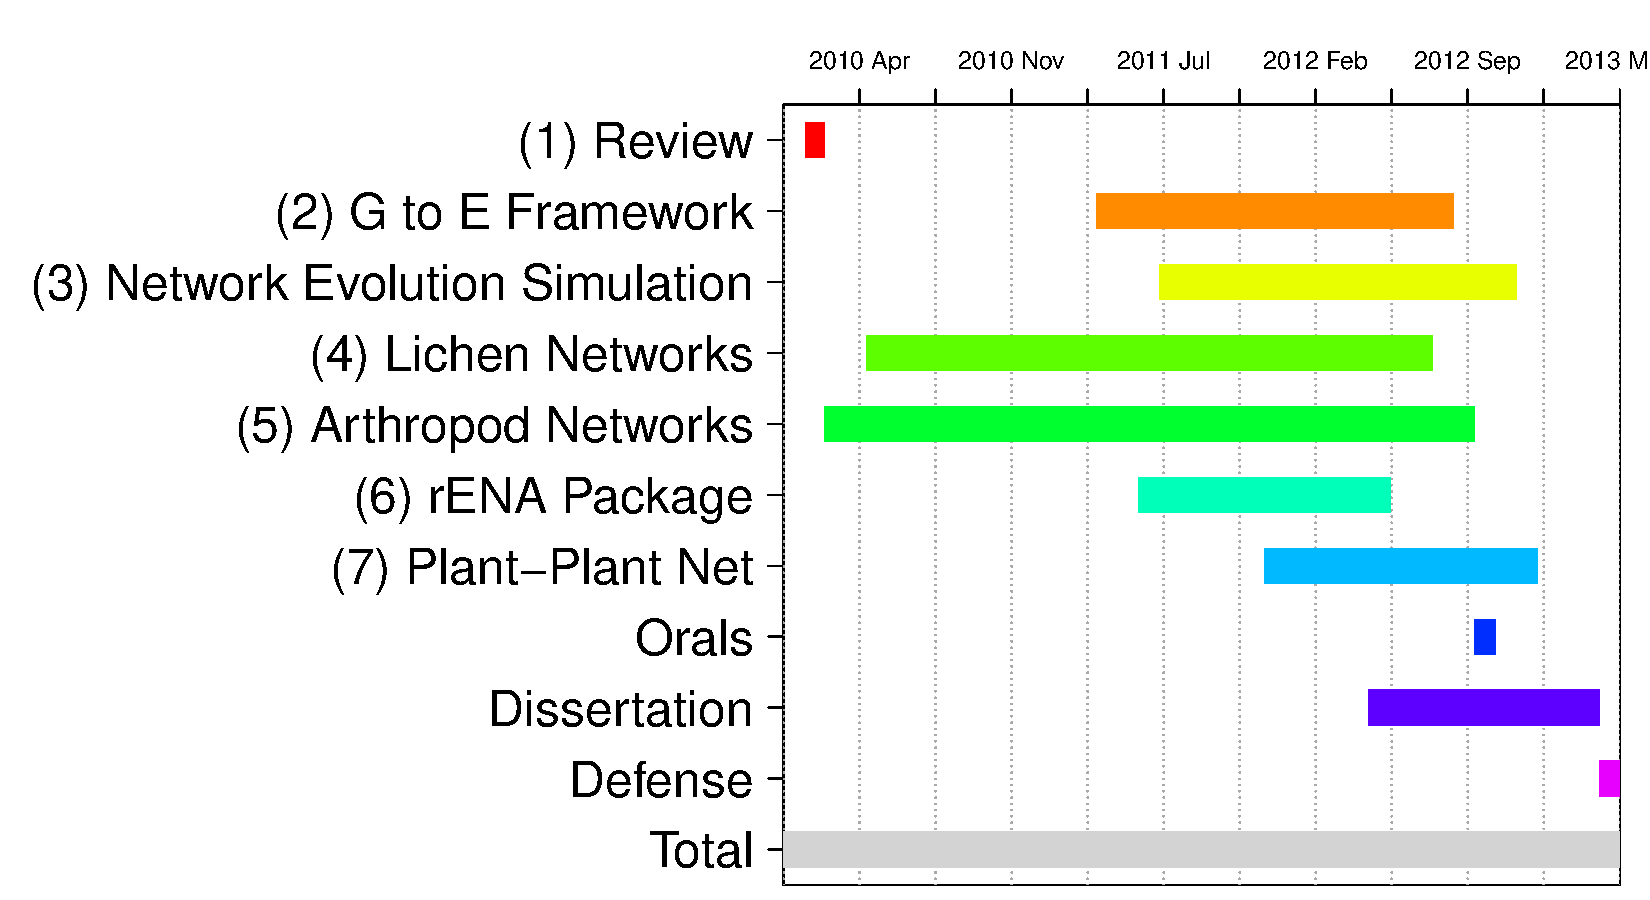
\includegraphics{meeting_notes_May2012-001}

%\section{References}
\bibliographystyle{nar}
\bibliography{/Users/Aeolus/Documents/bibtex/biblib}


\end{document}  


